\chapter{Примеры вычисления работы силы. Работа силы тяжести, линейной силы
упругости и силы тяготения.}

\section{Работа силы тяжести}
\begin{figure}[b]
    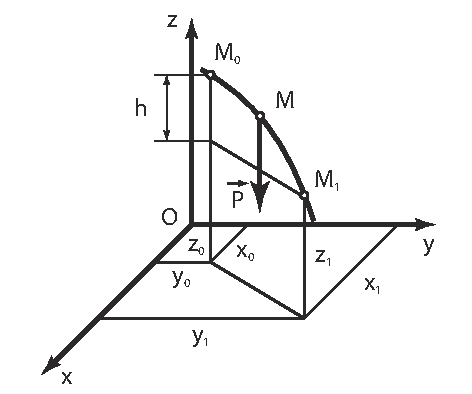
\includegraphics[width=.32\textwidth]{52_01}\hfill
    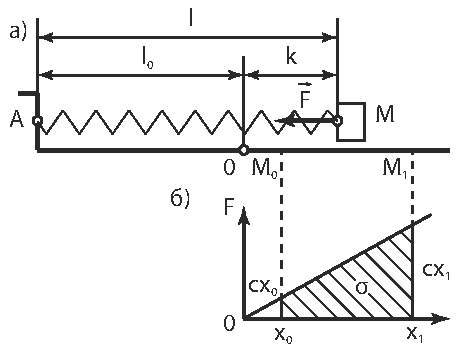
\includegraphics[width=.32\textwidth]{52_02}\hfill
    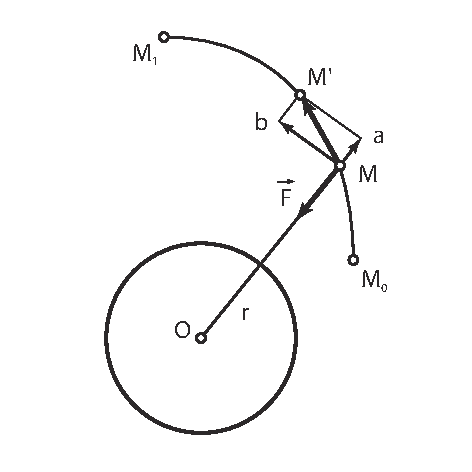
\includegraphics[width=.32\textwidth]{52_03}
    \parbox{.32\textwidth}{\caption{} \label{pic52_01}}\hfill
    \parbox{.32\textwidth}{\caption{} \label{pic52_02}}\hfill
    \parbox{.32\textwidth}{\caption{} \label{pic52_03}}
\end{figure}
Пусть точка \( M \), на которую действует сила тяжести \( \vec{P} \), 
перемещается из положения \( M_0(x_0, y_0, z_0) \) в положение 
\( M_1(x_1, y_1, z_1) \). Выберем координатные оси так, чтобы ось \( Oz \) 
была направлена вертикально вверх (рис.~\ref{pic52_01}). Тогда 
\( P_x = 0, P_y = 0, P_z = -P \). Подставляя эти значения в выражение для работы
\begin{equation}
    A = \int\limits_{(M_0)}^{(M_1)} F_x dx + F_y dy + F_z dz,
    \label{eq:1}    
\end{equation}
получим:
\[ 
    A = - \int\limits_{z_0}^{z_1} Pdz = 
    P\left(z_0 - z_1 \right).
\]
Из полученного результата следует, что работа силы тяжести не зависит от 
вида той траектории, по которой перемещается точка её приложения.

\section{Работа линейной силы упругости}
Рассмотрим груз \( M \), лежащий на горизонтальной плоскости и 
прикрепленный к свободному концу некоторой пружины (рис.~\ref{pic52_02}а). На 
плоскости отметим точку \( O \) положение, занимаемое концом пружины, 
когда она не напряжена (\( AO = l_0 \) -- длина ненапряженной пружины), и 
примем эту точку за начало координат. Если теперь оттянуть груз от 
равновесного положения \( O \), растянув пружину до величины \( l \), то
пружина получит удлинение \( \Delta l = l - l_0 \) и на груз будет действовать 
силу упругости \( \vec{F} \), направленная к точке \( O \). Так как в 
нашем случае \( \Delta l = |x| \), то по формуле \( F = c\Delta l \) 
(\( \Delta l \) -- удлинение (или сжатие) пружины, \( c \) -- коэффициент 
жёсткости пружины):
\[
    F = c\Delta l = c|x| \text{ и } F_x = -cx.
\]

Найдём работу, совершаемую силой упругости при перемещении груза из 
положения \( M_0(x_0) \) в положение \( M_1(x_1) \). Так как в данном 
случае \( F_x = -cx, F_y = F_z = 0 \), то, подставляя эти значения в 
формулу (\ref{eq:1}), найдём
\[ 
    A = - \int\limits_{x_0}^{x_1} cxdx = 
    \frac{c}{2} \left( x^{2}_0 - x^{2}_1 \right).
\]

\emph{Этот же результат можно получить по графику зависимости 
\( F \) от \( x \) (рис \ref{pic52_02}б), вычисляя площадь \( \sigma \) 
заштрихованной на чертеже трапеции и учитывая знак работы.}

В полученной формуле \( x_0 \) представляет собой начальное удлинение 
пружины, а \( x_1 \) -- конечное удлинение. 
Следовательно, 
\[
    A = \frac{c}{2} \left( k^{2}_0 - k^{2}_1 \right),
\]
то есть \emph{работа силы упругости равна половине произведения 
коэффициента жёсткости на разность квадратов начального и конечного 
удлинения (или сжатий) пружины.}

\section{Работа силы тяготения}
Если Землю (планету) рассматривать как однородный шар (или шар, 
состоящий из однородных концентрических слоёв), то на точку \( M \) с 
массой \( m \), находящуюся вне шара на расстоянии \( r \) от его 
центра \( O \) (или находящуюся на поверхности шара), будет действовать 
сила тяготения \( \vec{F} \), направленная к центру \( O \)
(рис.~\ref{pic52_03}), значение которой определяется формулой 
\[
    F = \frac{km}{r^2}.
\]
Коэффициент \( k \) определим из того условия, что, когда точка 
находится на поверхности планеты (\( r = R \), где \( R \) -- радиус планеты), 
сила притяжения равна \( mg \), где \( g \) -- ускорение силы тяжести 
(точнее силы тяготения) на земной поверхности. Тогда должно быть
\[ mg = \frac{km}{R^2} \text{ и } k = gR^2 \]

Подсчитаем сначала элементарную работу силы \( \vec{F} \). Разложим элементарное
перемещение на радиальную и касательную составляющую. Так как гравитационное
поле в рассматриваемом случае радиально, то сила гравитационного взаимодействия
имеет только радиальную составляющую:
\[
    dA = -Fdr = -km\frac{dr}{r^2} = -mgR^2 \frac{dr}{r^2}.
\]

Допустим теперь, что точка перемещается из положения \( M_0 \), где 
\( r = r_0 \), в положение \( M_1 \), где \( r = r_1 \). Тогда 
\[ 
    A = \int\limits_{(M_0)}^{(M_1)} dA = 
    -mgR^2 \int\limits_{r_0}^{r_1} \frac{dr}{r^2} =
    mgR^2 \int\limits_{r_0}^{r_1} d\left( \frac{1}{r} \right)
\]
или окончательно
\[
    A = mgR^2 \left( \frac{1}{r_1} - \frac{1}{r_0} \right).
\]

\newpage
